\section{Scheduling}
\subsection{Implementation Breakdown}
The scheduler simulates a multi-processing environment where CPU time must be divided fairly among competing processes. It relies on two core modules: \texttt{queue.c} for priority-based ready queue management and \texttt{sched.c} for the complex scheduling logic.

\subsubsection{Ready Queue Management (\texttt{queue.c})}
The ready queues are implemented as separate arrays of \texttt{pcb\_t} structs, allocating one queue per priority level. This avoids sorting overhead when enqueuing processes.
\begin{itemize}
    \item \textbf{\texttt{enqueue(q, proc):}} Appends a PCB to the end of the array. The time complexity is $\mathcal{O}(1)$. This ensures that inserting a process into the system is incredibly fast. A guard check ensures the queue does not exceed \texttt{MAX\_QUEUE\_SIZE}.
    \item \textbf{\texttt{dequeue(q):}} Removes a process from the front (FIFO order). Since it's implemented via arrays rather than linked lists, removing an element requires shifting the remaining elements left, leading to an $\mathcal{O}(n)$ time complexity.
    \item \textbf{\texttt{purgequeue(q, proc):}} Iterates over the queue to find a specific \texttt{pcb\_t*} \textbf{pointer} (not a PID) and removes it. Internally it uses pointer equality (\texttt{q->proc[i] == proc}). It also operates in $\mathcal{O}(n)$ time. PID-based lookup is handled by the separate \texttt{find\_proc\_by\_pid()} function in \texttt{sched.c}.
\end{itemize}

\subsubsection{Scheduling Logic (\texttt{sched.c})}
The operating system implements a strict \textbf{Multi-Level Queue (MLQ)} algorithm, maintaining 140 different priority levels (\texttt{MAX\_PRIO = 140}).

\begin{lstlisting}[language=C, caption=Scheduler Definitions]
static struct queue_t ready_queue; // legacy queue
static struct queue_t run_queue;   // legacy run queue (obsoleted)
static struct queue_t running_list;// currently dispatched processes
static pthread_mutex_t queue_lock; // synchronization mutex

#ifdef MLQ_SCHED
static struct queue_t mlq_ready_queue[MAX_PRIO]; 
static int slot[MAX_PRIO]; // Remaining CPU slots for each queue
#endif
\end{lstlisting}

\begin{theorybox}[The \texttt{slot} Budgeting System]
Unlike simple Priority Scheduling which causes severe starvation for low-priority processes, our MLQ policy allocates a specific \texttt{slot} (time budget) to each priority queue. The number of slots is calculated as \texttt{MAX\_PRIO - prio}. A queue can only dispatch processes until its slots run out. Once empty, it is locked out until all other non-empty queues also deplete their slots, forcing the system to give lower-priority queues a chance to execute.

\textbf{Example:} Priority 0 (highest) receives $140 - 0 = 140$ slots. Priority 139 (lowest) receives $140 - 139 = 1$ slot. This ensures priority 0 gets 140 times more CPU opportunities per cycle than priority 139, but priority 139 is \textit{never starved} entirely.
\end{theorybox}

The logic revolves around three core functions:
\begin{itemize}
    \item \textbf{\texttt{add\_mlq\_proc(proc):}} Inserts a newly created process directly into its respective priority queue (\texttt{mlq\_ready\_queue[proc->prio]}). Since this process has just been loaded by the system and has never been executed, there is no need to check or remove it from the \texttt{running\_list}. Before enqueuing, it sets up the kernel structure pointers (\texttt{proc->krnl->ready\_queue}, \texttt{proc->krnl->mlq\_ready\_queue}, \texttt{proc->krnl->running\_list}) so that later system call handlers can access the scheduler queues.
    \item \textbf{\texttt{get\_mlq\_proc():}} Scans from priority 0 (highest) to 139 (lowest). It finds the highest priority queue that is both non-empty and has \texttt{slot > 0}. It dequeues a process, decrements the slot counter, and adds it to the \texttt{running\_list}.
    \item \textbf{\texttt{put\_mlq\_proc(proc):}} When a process uses up its time slice, the CPU interrupts it. This function removes the process from \texttt{running\_list} and pushes it to the back of its priority queue to maintain Round-Robin fairness. It also refreshes the kernel structure pointers, identically to \texttt{add\_mlq\_proc}.
\end{itemize}

\subsection{Code Walkthrough: \texttt{get\_mlq\_proc()}}
Let's analyze the precise code that fetches the next process.
\begin{lstlisting}[language=C, caption=\texttt{get\_mlq\_proc} Implementation]
struct pcb_t *get_mlq_proc(void)
{
	struct pcb_t *proc = NULL;

	pthread_mutex_lock(&queue_lock);
	{
		int i;
		int has_ready = 0;
		int selected_prio = -1;

		for (i = 0; i < MAX_PRIO; i++) {
			if (!empty(&mlq_ready_queue[i])) {
				has_ready = 1;
				if (slot[i] > 0) {
					selected_prio = i;
					break; 
				}
			}
		}

		if (selected_prio == -1 && has_ready) {
			for (i = 0; i < MAX_PRIO; i++)
				slot[i] = MAX_PRIO - i; 

			for (i = 0; i < MAX_PRIO; i++) {
				if (!empty(&mlq_ready_queue[i])) {
					selected_prio = i;
					break;
				}
			}
		}

		if (selected_prio != -1) {
			proc = dequeue(&mlq_ready_queue[selected_prio]);
			slot[selected_prio]--; 
			enqueue(&running_list, proc);
		}
	}
	pthread_mutex_unlock(&queue_lock);

	return proc;
}
\end{lstlisting}
\textbf{Analysis:} The outer loop checks from \texttt{i = 0} upwards. It finds the first queue that has processes and still has a positive \texttt{slot[i]}. The flag \texttt{has\_ready} tracks whether any queue has waiting processes. Crucially, if \texttt{selected\_prio} remains $-1$ but \texttt{has\_ready} is true, it means all active queues have exhausted their slot budgets. The scheduler immediately resets every slot back to \texttt{MAX\_PRIO - i} and retries the fetch. This reset cycle is the mechanism that guarantees starvation prevention.

\subsection{Kernel Structure Pointer Setup}
Both \texttt{add\_mlq\_proc} and \texttt{put\_mlq\_proc} configure the process's kernel structure pointers before enqueuing. This is critical because system call handlers (e.g., \texttt{\_\_sys\_memmap}) need access to the scheduler's queues to locate processes by PID:
\begin{lstlisting}[language=C, caption=Kernel pointer configuration in \texttt{put\_mlq\_proc}]
void put_mlq_proc(struct pcb_t *proc) {
    proc->krnl->ready_queue = &ready_queue;
    proc->krnl->mlq_ready_queue = mlq_ready_queue;
    proc->krnl->running_list = &running_list;

    pthread_mutex_lock(&queue_lock);
    purgequeue(&running_list, proc);
    enqueue(&mlq_ready_queue[proc->prio], proc);
    pthread_mutex_unlock(&queue_lock);
}
\end{lstlisting}
Without this step, the \texttt{find\_proc\_by\_pid()} function called from within kernel-mode system calls would not be able to traverse the scheduler queues to resolve a process PID to its \texttt{pcb\_t} structure.

\subsection{Thread Safety}
Since this OS supports multiple simulated CPUs concurrently fetching and putting processes, every queue modification is enclosed in \texttt{pthread\_mutex\_lock(\&queue\_lock)} and \texttt{pthread\_mutex\_unlock(\&queue\_lock)}. This prevents race conditions where two CPUs might dequeue the exact same \texttt{pcb\_t} block, leading to catastrophic kernel crashes.

\subsection{Gantt Diagram}
By running the system against \texttt{sched.input}, \texttt{sched\_0.input}, and \texttt{sched\_1.input}, we observe the execution flow across the available virtual CPUs.
\begin{figure}[H]
    \centering
    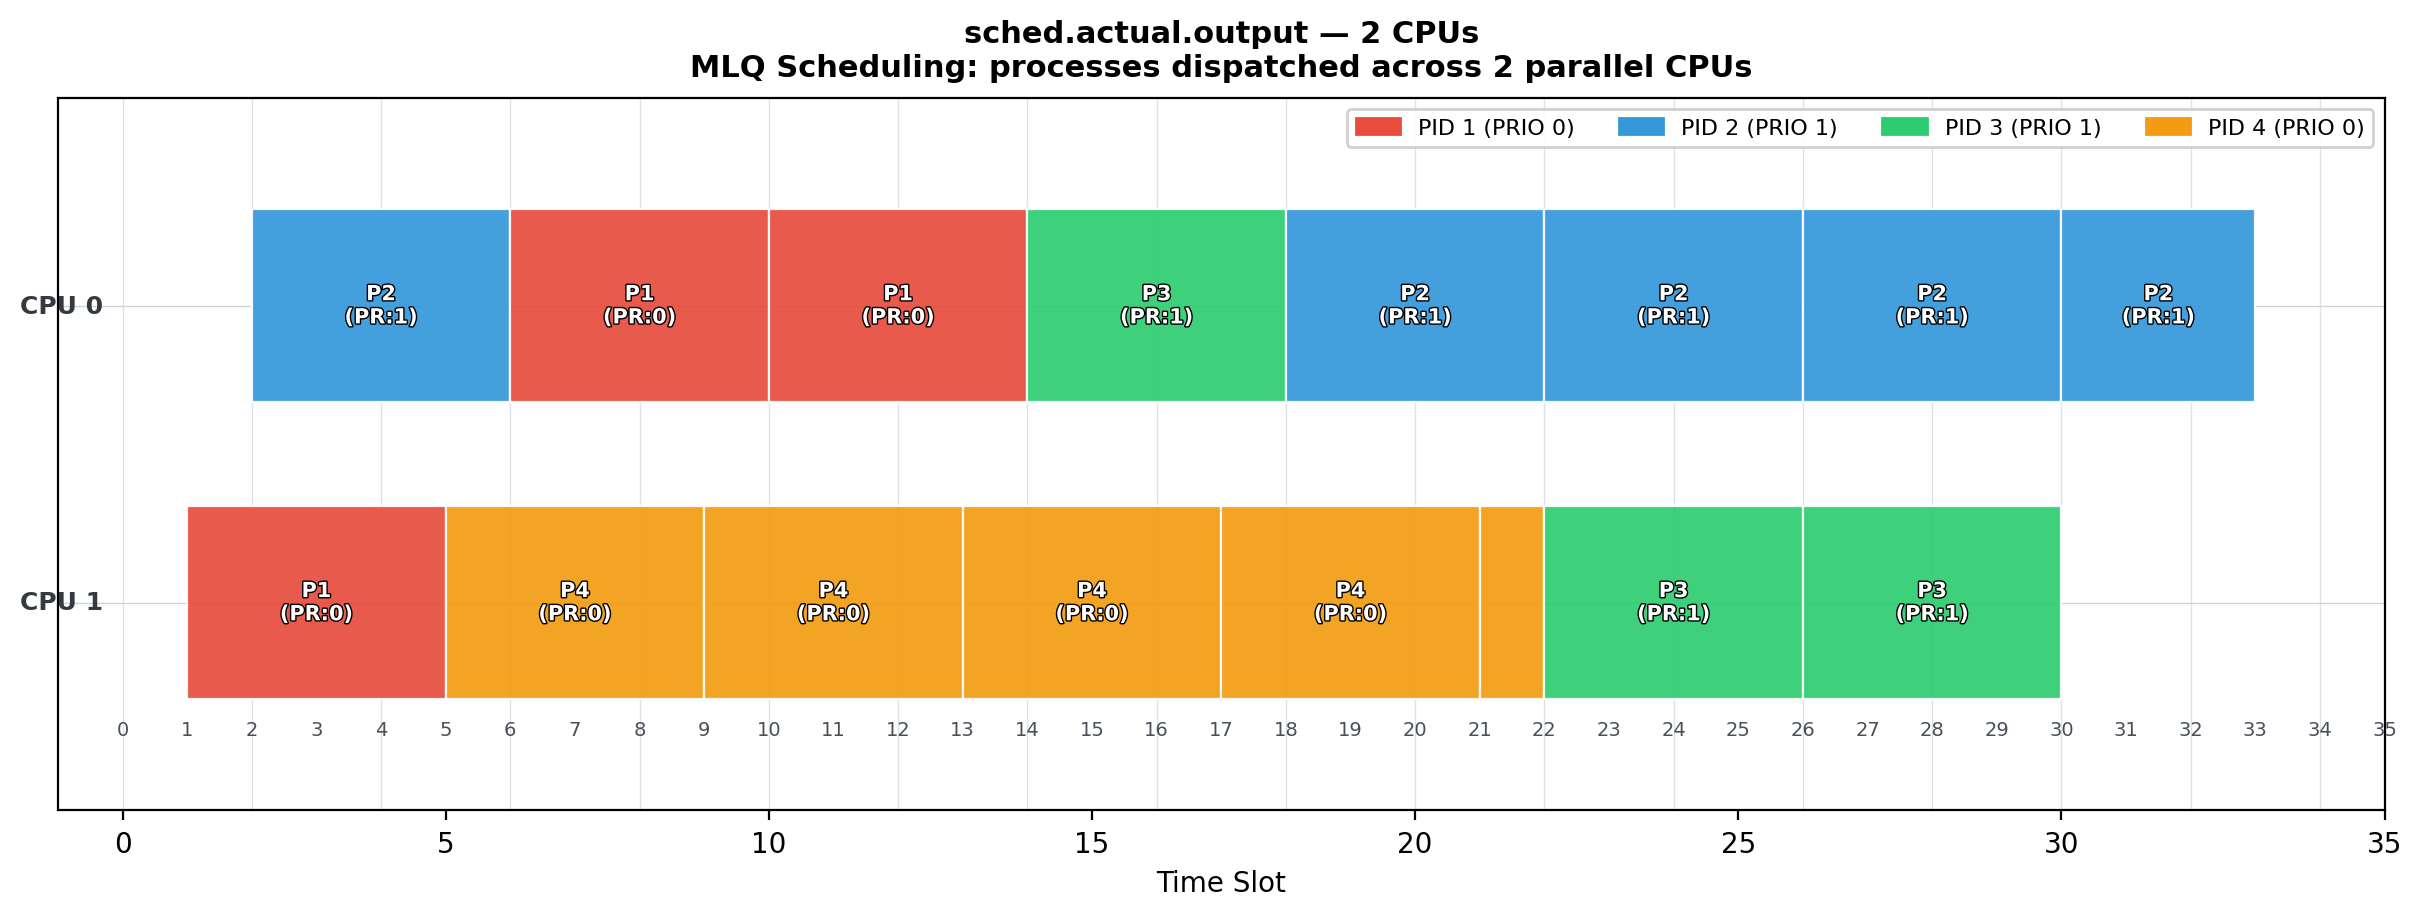
\includegraphics[width=0.8\linewidth]{Images/gantt_sched.png}
    \caption{Gantt Diagram Execution Trace of \texttt{sched.input} (2 CPUs)}
\end{figure}
\begin{figure}[H]
    \centering
    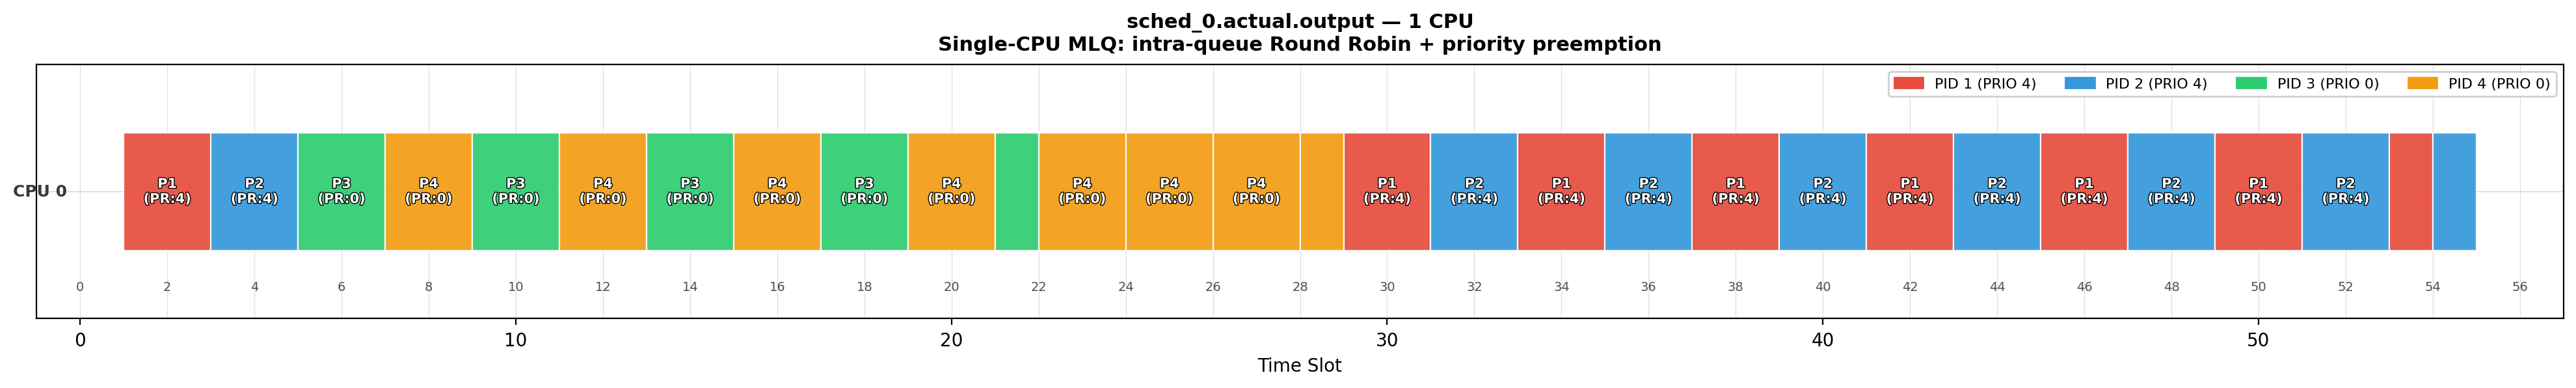
\includegraphics[width=1\linewidth]{Images/gantt_sched_0.png}
    \caption{Gantt Diagram Execution Trace of \texttt{sched\_0.input} (1 CPU)}
\end{figure}
\begin{figure}[H]
    \centering
    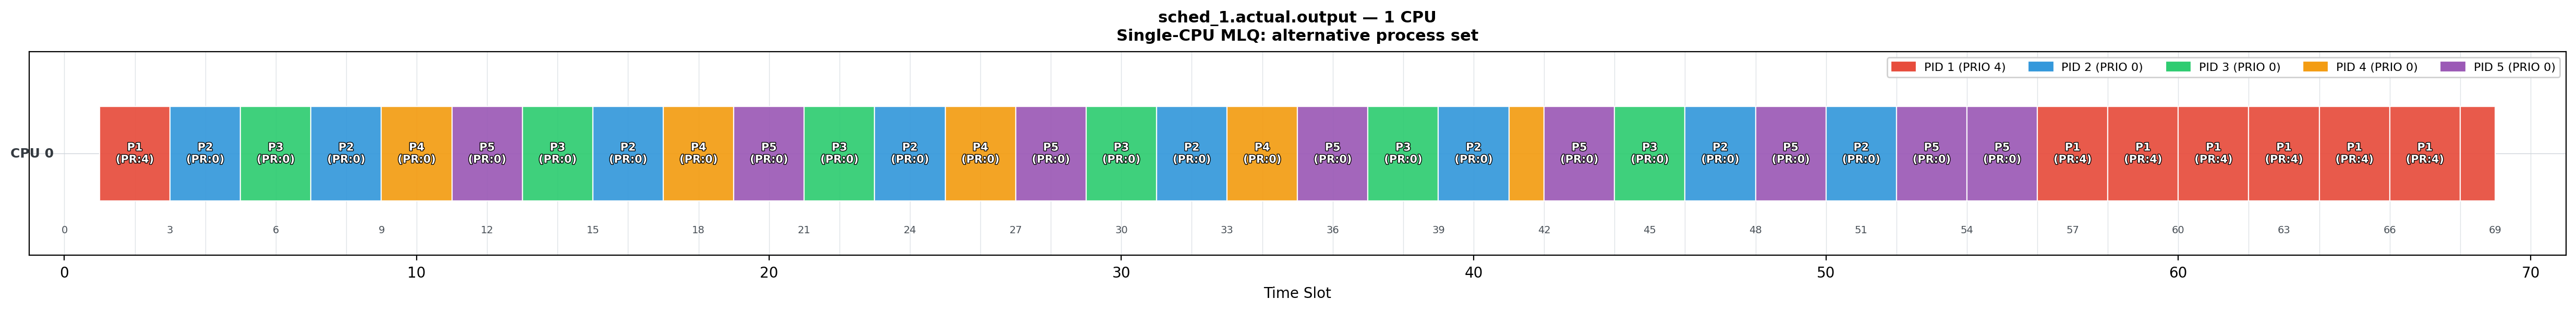
\includegraphics[width=1\linewidth]{Images/gantt_sched_1.png}
    \caption{Gantt Diagram Execution Trace of \texttt{sched\_1.input} (1 CPU)}
\end{figure}